\chapter{Technical Design}
\begin{comment}
    # Universal Design (Universal Utforming)
    # OpenLayers vs Leaflet (or others)
    # Openlayers TileWMS vs ImageWMS (optimalisering av kartet)
\end{comment}

\section{System Architecture}\label{sec:systemarchitecture}
% client-server model, microservices, layers of the application ? 

\section{Data Flow} % e.g., how user requests move through the system).

TEMP LOKASJON

% KANSKJE ENDRE "ocean and fjord" og "Glacial river" til "Marine" og "glaciofluvial" slik det er brukt i introduksjon.
\begin{figure}[h]
    \centering
    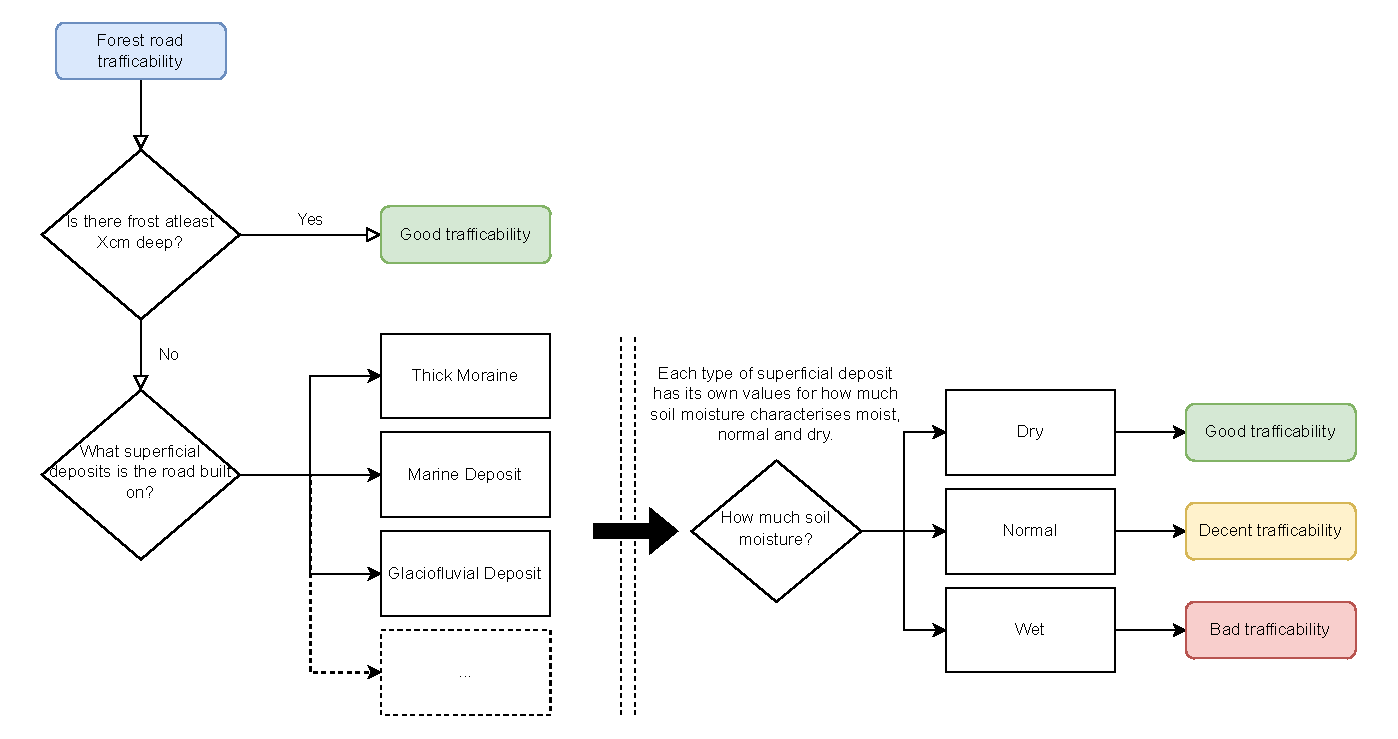
\includegraphics[width=1\linewidth]{figures/roadclassification.pdf}
    \caption[Diagram visualizing the forest road classification.]{xx}
    \label{fig:forestroadclassification}
\end{figure}
% (fra diagram) How much soil moisture, kommer an på permeability

\section{Sequence Diagram}
\begin{figure}[h]
    \centering
    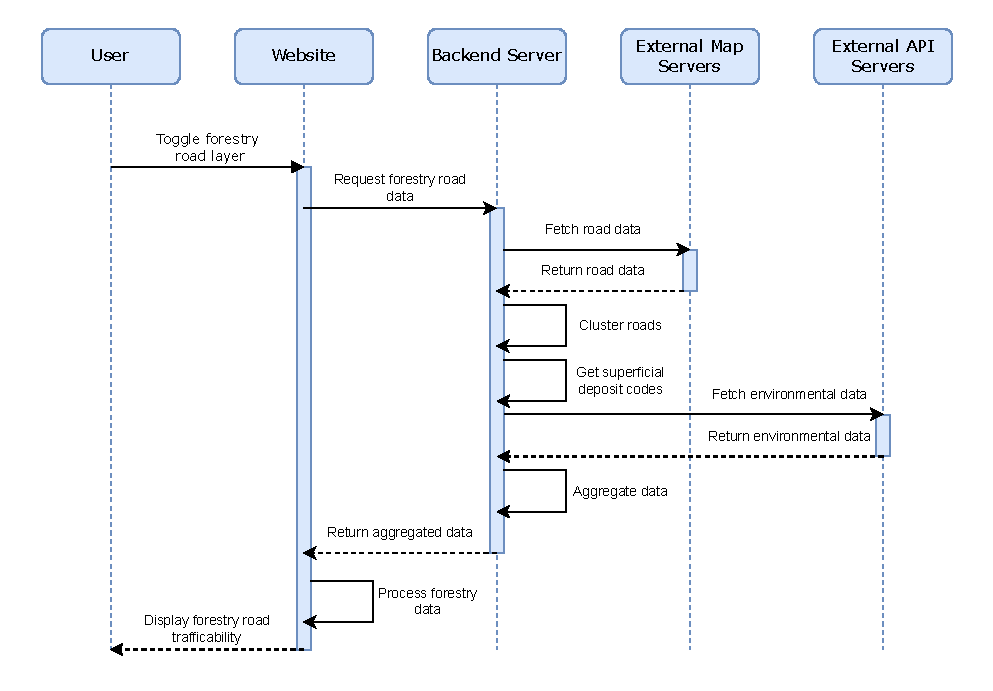
\includegraphics[width=1\linewidth]{figures/sequence_diagram.pdf}
    \caption{Sequence diagram of forestry road map layer}
    \label{fig:sequence_diagram}
\end{figure}

\hyperref[fig:sequence_diagram]{Figure \ref*{fig:sequence_diagram}} shows the sequence diagram for when the user toggles the forestry road map layer. The whole sequence consists of these steps:
\begin{enumerate}
    \item \textbf{Toggle forestry road layer}: The user toggles the forestry road map layer on the website.
    \item \textbf{Request forestry road data}: The website sends a request to the backend server for the necessary data within the visible map area.
    \item \textbf{Fetch road and weather data}: The backend server, acting as a proxy, fetches the required road and weather data from external map servers.
    \item \textbf{Return road and weather data}: The map servers return the requested road and weather data.
    \item \textbf{Aggregate data}: The backend server aggregates the data into a single payload.
    \item \textbf{Return aggregated data}: The backend server sends the aggregated data back to the website.
    \item \textbf{Process forestry data}: The website processes the data and determines the trafficability of roads within the visible map area.
    \item \textbf{Display forestry road trafficability}: The forestry road layer, including trafficability, is rendered on the user's map.
\end{enumerate}

\section{Website}
The website serves as the user interface of the system, allowing users to visualize and interact with data related to forestry road conditions and weather-based forecasts using a dynamic map.

The system follows a client-server architecture, where the website acts as a client and communicates with a backend server via a REST API. The processing of meteorological and geological data is handled on the server side. The frontend is responsible for requesting data, rendering maps, and presenting relevant information to the user.

The classification of road trafficability is performed on the client side, as the website allows users to dynamically adjust thresholds for certain meteorological and geological parameters. Normally, this would be handled entirely by the backend server, but in order to provide immediate feedback when the user changes these thresholds, the classification logic is implemented in the frontend. This hybrid approach ensures a responsive user experience while keeping the most computationally expensive operations on the server.

The interaction between the website and the server is stateless, meaning that each request is independent and contains all the information needed to process it. This architectural choice improves system robustness and simplifies both development and deployment, particularly when it comes to scaling.

A central component of the website is its interactive map interface, which displays spatial data such as forestry road networks, map layers, and calculated trafficability classifications. The map is rendered dynamically in the browser using client-side resources, and data is loaded based on the user’s current viewport and zoom level. This approach ensures efficient data usage and good performance, even when dealing with large or detailed geographic datasets.

The website is implemented as a single-page application (SPA), where all rendering and interface updates occur dynamically without full page reloads. This enables smooth interaction and better performance, as only relevant parts of the page are updated via the Document Object Model (DOM). \acrshort{html} 5 is required for full functionality, and the system relies on an active internet connection to fetch data from the server and external services. While the system is primarily intended for desktop and laptop use, it also runs on mobile devices, though the \acrshort{ui} is not optimized for smaller screens.

Choosing to implement the frontend as a web application provides several benefits. It ensures accessibility across a wide range of devices without the need for local installation, making the tool usable both in office environments and in the field.

Overall, the design of the website emphasizes a clean separation of concerns, efficiency in data handling, and accessibility, which together form a robust and user-friendly frontend component for the system.

\subsection{Map Layers}
% KANKJE GLOSSARY FOR "COMPOSITE MAP"
The interactive map on the website supports multiple layers, allowing the user to build a composite map with various types of data. These layers include both meteorological and geological information relevant to assessing road conditions and the surrounding environment.

\subsubsection*{Base Layers}
The user has the option to change the base layer of the map. In the current version, two options are available: the standard map from \Gls{openstreetmap}\footnote{\url{https://www.openstreetmap.org}} and the terrain map from OpenTopoMap\footnote{\url{https://opentopomap.org}}.
% KANSKJE GI GRUNN TIL HVORFOR DET IKKE KUN ER ETT BASE LAYER VALG

\begin{figure}[h]
     \centering
     \begin{subfigure}[b]{0.45\textwidth}
         \centering
         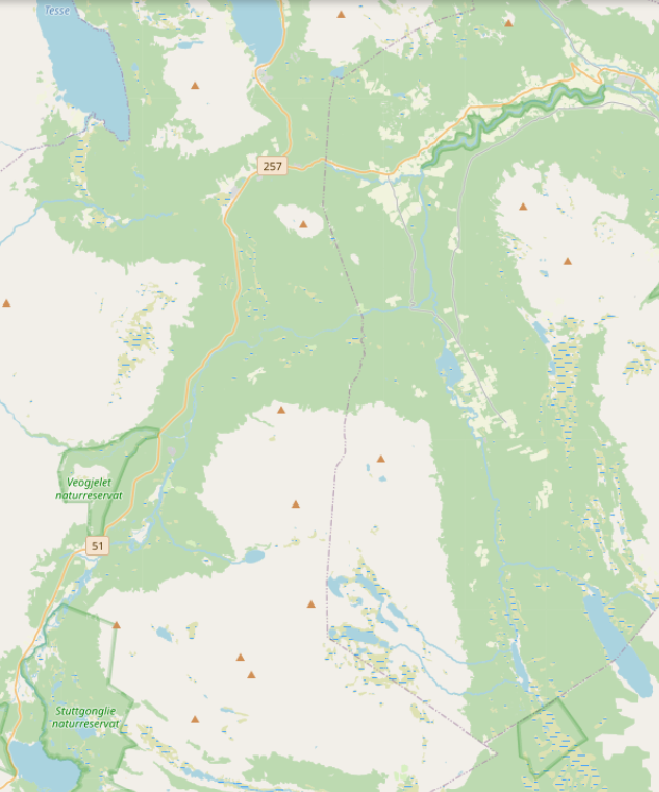
\includegraphics[width=\textwidth]{figures/base_layer_standard.pdf}
         \caption{Standard base layer}
         \label{fig:base_layer_standard}
     \end{subfigure}
     \hfill
     \begin{subfigure}[b]{0.45\textwidth}
         \centering
         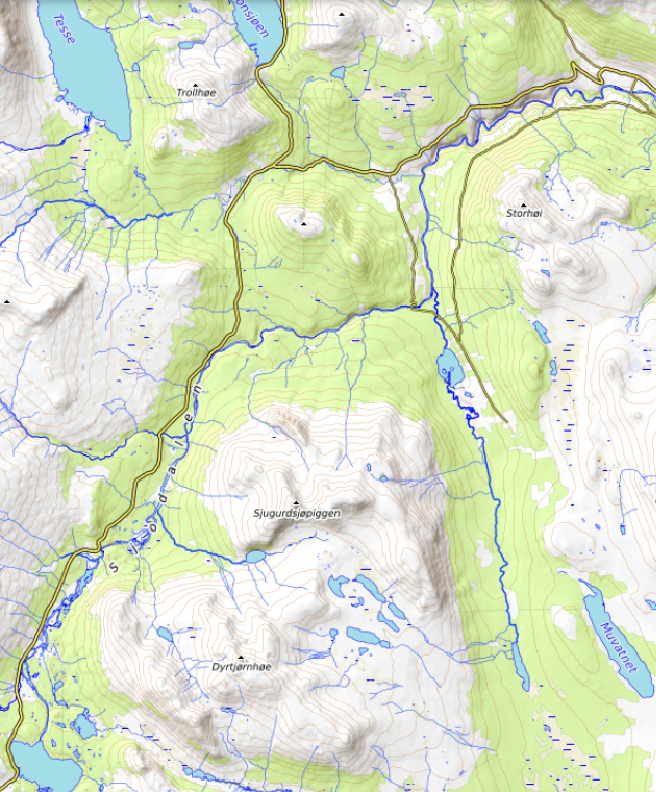
\includegraphics[width=\textwidth]{figures/base_layer_topo.pdf}
         \caption{Terrain base layer}
         \label{fig:base_layer_topo}
     \end{subfigure}
    \caption{Base map layer options}
    \label{fig:base_layers}
\end{figure}

\subsubsection*{Superficial Deposits}
% LEGGE INN FARGE KODER FOR LØSMASSETYPE. TRENGER IKKE FOR ALLE? KANSKJE VEDLEGG?
The map layer showing superficial deposits is provided by \acrshort{ngu}. The superficial deposits data provide information on the distribution of surface sediments covering bedrock, mainly formed during and after the last Ice Age. It represents the dominant soil type in the upper layers, but does not account for deeper variations. These soil types include stones, gravel, sand, clay, peat, and moraine material \cite{geonorge_losmasser}. 

\begin{figure}[h]
    \centering
    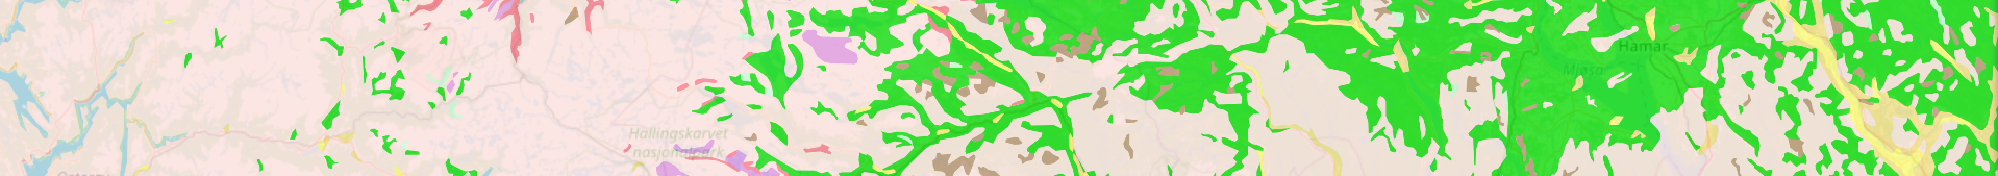
\includegraphics[width=1\linewidth]{figures/losmasse_eksempel.pdf}
    \caption{Example of the superficial deposits map layer}
    \label{fig:superficial_deposit_example}
\end{figure}

\subsubsection*{Frost Depth}
% Kanskje nevn GWB modellen? https://www.senorge.no/WaterMap
The frost depth map layer is provided by \acrshort{nve}. It shows the frost depth as a raster-based map ranging from very deep frost (dark blue) to no frost (light green). Looking at frost depth can make it easy to determine the trafficability of forestry roads. As long as there is frost, i.e. 10 cm or deeper (see \hyperref[tab:frost_depth_classification]{Table \ref*{tab:frost_depth_classification}}) all roads good to drive on. Therefore most of the forestry roads during the Norwegian winter would have good trafficability.

% KANSKJE GI EKSEMPLER PÅ NÅR (OG HVOR) DET ER VANLIG MED DE FORSKJELLIGE DYBDENE
\begin{table}[h]
    \centering
    \begin{tabular}{|l|l|l|}
        \hline  
        Color & Frost Depth & Depth in cm \\
        \hline
        \cellcolor[HTML]{00009c} & Very Deep Frost & > 75 cm \\
        \hline
        \cellcolor[HTML]{0018ff} & Deep Frost & 30-75 cm \\
        \hline
        \cellcolor[HTML]{009aff} & Frost & 10-30 cm \\
        \hline
        \cellcolor[HTML]{84ebff} & Shallow Frost & 5-10 cm \\
        \hline
        \cellcolor[HTML]{deffff} & Partially Frost-free & 0-5 cm \\
        \hline
        \cellcolor[HTML]{cef77b} & No Frost & 0 cm \\
        \hline
    \end{tabular}
    \caption{Frost depth classification and corresponding colors \cite{nve2025waterdata}}
    \label{tab:frost_depth_classification}
\end{table}

\begin{figure}[h]
    \centering
    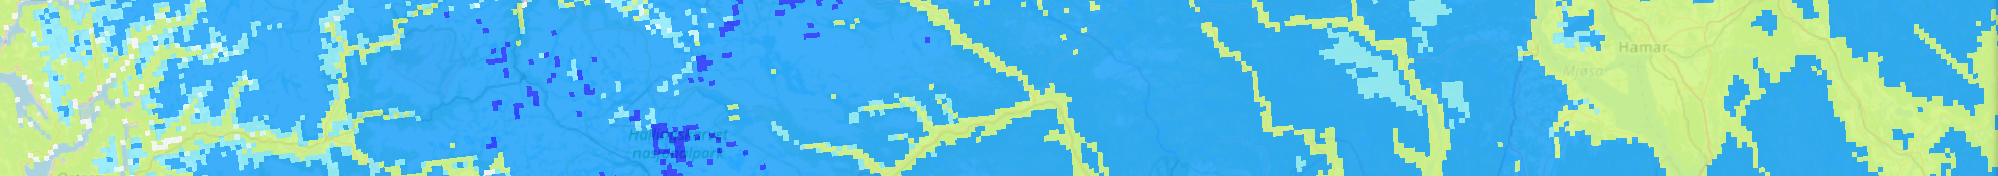
\includegraphics[width=1\linewidth]{figures/teledyp_eksempel.pdf}
    \caption{Example of the frost depth map layer}
    \label{fig:frost_depth_example}
\end{figure}

\subsubsection*{Soil Saturation}

\subsubsection*{Forestry Roads}
The forestry roads map layer is a vector layer which is retrieved from a WFS, provided by GeoNorge and Kartverket. The roads are shown in the colors, green, yellow, or red, depending on their trafficability, which is calculated using meteorological and geological data as factors. 

\subsubsection*{Sources of Uncertainty}
There are some sources of error in the water maps, i.e. the frost depth and soil saturation maps. Errors may arise from inaccuracies in the interpolation of these variables or from the model interpreting conditions differently than they actually are. This is especially critical when the temperature is around 0\textdegree C, where small differences can determine whether precipitation falls as rain or snow, or whether snow melts. Local rain showers that aren't captured by weather stations may also be missed. Furthermore, factors like wind, humidity, and solar radiation— which aren't included in the model—can lead to significantly more snowmelt in reality. The maps in SeNorge and Xgeo typically show daily averages, which means they may miss short-term variations like heavy rain or temperature swings within a day. However, Xgeo also provides 3-hourly maps that better reflect intraday changes. Forecast maps extend up to nine days ahead, based on the same weather models as those used on Yr, with increasing uncertainty the further ahead they go. Additionally, the model may not perfectly represent vegetation or soil conditions, potentially leading to over- or underestimation of water saturation and groundwater levels. \cite{senorge_watermap}

\subsection{Folder Structure}
\begin{figure}[h]
    \centering
    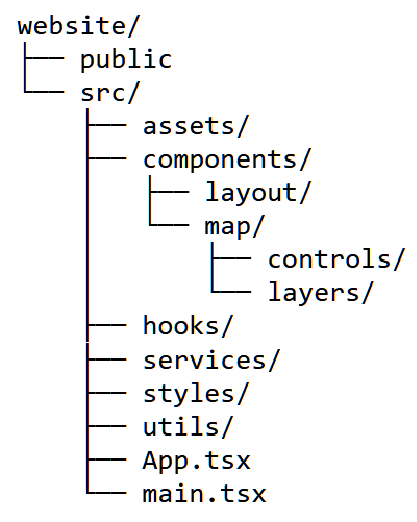
\includegraphics[width=0.5\linewidth]{figures/website_folder_structure.pdf}
    \caption{Folder structure of the website}
    \label{fig:website_folder_structure}
\end{figure}

\section{Server}
\subsection{Golang?/Libraries}
\subsection{Map and Weather Services} % endre navn?
% Lag tabell e.l. av alle services som brukes (WMS/API) ?
Multiple map services were used in this project to ultimately determine the trafficability of forestry roads. Retrieving data from WMS and WFS was made easy with OpenLayers as it includes functions for this. 
\subsubsection*{Frost Depth}
% KANSKJE HA ENDA MED DETALJER? WMS PARAMETER (LAYERS, etc.)
% SPESIFISER LOKASJON 
\begin{table}[h]
    \centering
    \begin{tabularx}{\linewidth}{|l|X|}
        \hline
        \textbf{Service Type:} & \Gls{wms} \\
        \hline
        \textbf{Data Provided:} & \Gls{frost} Depth (1 x 1 km Resolution) \\
        \hline
        \textbf{Data Format:} & PNG \\
        \hline
        \textbf{Data Source:} & \Gls{nve} \\
        \hline
        \textbf{URL:} & \url{} \\
        \hline
        \textbf{Rate Limit:} & No Limit \\
        \hline
        \textbf{Authorization:} & No Authorization Needed \\
        \hline
    \end{tabularx}
    \caption{Details about frost depth map service}
    \label{tab:frost_map_service}
\end{table}


\subsubsection*{Soil Moisture}
\begin{table}[h]
    \centering
    \begin{tabularx}{\linewidth}{|l|X|}
        \hline
        \textbf{Service Type:} &  \\
        \hline
        \textbf{Data Provided:} &  \\
        \hline
        \textbf{Data Format:} &  \\
        \hline
        \textbf{Data Source:} &  \\
        \hline
        \textbf{URL:} &  \\
        \hline
        \textbf{Rate Limit:} &  \\
        \hline
        \textbf{Authorization:} & \\
        \hline
    \end{tabularx}
    \caption{Details about soil moisture map service}
    \label{tab:soil_moisture_map_service}
\end{table}

\subsubsection*{Superficial Deposits}
\begin{table}[h]
    \centering
    \begin{tabularx}{\linewidth}{|l|X|}
        \hline
        \textbf{Service Type:} & \Gls{wms} \\
        \hline
        \textbf{Data Provided:} & Superficial Deposits (Scale: 1:1,000,000 and 1:20,000) \\
        \hline
        \textbf{Data Format:} & PNG \\
        \hline
        \textbf{Data Source:} & \acrshort{ngu} \\
        \hline
        \textbf{URL:} &  \\
        \hline
        \textbf{Rate Limit:} & No Limit \\
        \hline
        \textbf{Authorization:} & No Authorization Needed\\
        \hline
    \end{tabularx}
    \caption{Details about superficial deposit map service}
    \label{tab:superficial_deposit_map_service}
\end{table}

\subsubsection*{Forestry Roads}
\begin{table}[h]
    \centering
    \begin{tabularx}{\linewidth}{|l|X|}
        \hline
        \textbf{Service Type:} & WFS \\
        \hline
        \textbf{Data Provided:} & Forestry Roads \\
        \hline
        \textbf{Data Format:} & \Gls{geojson} \\
        \hline
        \textbf{Data Source:} & Geonorge and Kartverket \\
        \hline
        \textbf{URL:} &  \\
        \hline
        \textbf{Rate Limit:} &  \\
        \hline
        \textbf{Authorization:} & No Authorization Needed \\
        \hline
    \end{tabularx}
    \caption{Details about forestry road map service}
    \label{tab:forestry_road_map_service}
\end{table}


\subsection{Map Data Processing}
\begin{comment}
    # Concurrency (works with multiple cores, might be slower with one core?)
\end{comment}

% ANDRE DIAGRAM? sequence diagrams, component diagrams, etc.